\chapter{OpenCms User Manual}
\label{OpenCms User Manual}

\section{Introduction}

\subsection{What is OpenCms?}

OpenCms 5 is a Content Management System that is based on Open
Source Software. Complex Intranet and Internet websites can be
quickly and cost-effectively created, maintained and managed.

OpenCms enables you to create complete websites offline that are
published when you're satisfied with the results. An offline
project enables several users with different permissions to work
on the offline version as a team. OpenCms enables you to easily
coordinate users that are writing, designing or managing content.
It also enables you to manage the project's workflows.

Once it has been completed and approved, the offline version is
published by the project manager. Subsequent modifications and
maintenance activities are performed offline. The site is updated
by replacing the online files with the files that were modified
offline.

\subsection{The advantages of OpenCms}

OpenCms is platform independent. The software used to create the
website is installed on a web server and is accessed via the
Internet from any location such as your home. Users use their web
Browser to access OpenCms via the Internet. The combination of
their user name and password ensures that their work environment
remains protected. All of the web server's software components are
based on Java technology.

\subsection{Configuring the client}

Netscape Navigator or Microsoft Internet Explorer must be
installed on the client. You should use IE 5.5 or higher or
Netscape Navigator 7.0 or higher. Configuration details for each of
the Browsers can be found in chapter \ref{Client Setup}. 

We divided the user's guide, which explains how to use the system's
most important functions, into two sections: Section 1 consists of a
demo that is intended to give you a practical introduction to
OpenCms; Section 2 describes the individual functions of OpenCms 
more detailed.

\textbf{NOTE:} Our explanations are based on the assumption that
OpenCms has been successfully installed and is running on your web
server or local computer.

\newpage
\section{Section 1: OpenCms - The demo}

The following demo is based on a real life scenario and was
designed to get you up and running as quickly as possible.
The module \texttt{org.opencms.welcome} must be present in your OpenCms system
(it is installed per default by the OpenCms setup).

Open your Internet browser and enter

{\tt http://localhost:8080/opencms/opencms/}

to access the OpenCms welcome site.

The OpenCms site welcome page is displayed (Figure~\ref{demopage01}). The navigator on top contains
the links to all of the pages. Click on "Release notes".

The release notes page is displayed. The first
section of the demo consists of modifying this page in OpenCms by
following the instructions described below.

\begin{figure}[!hbt]
\begin{center}
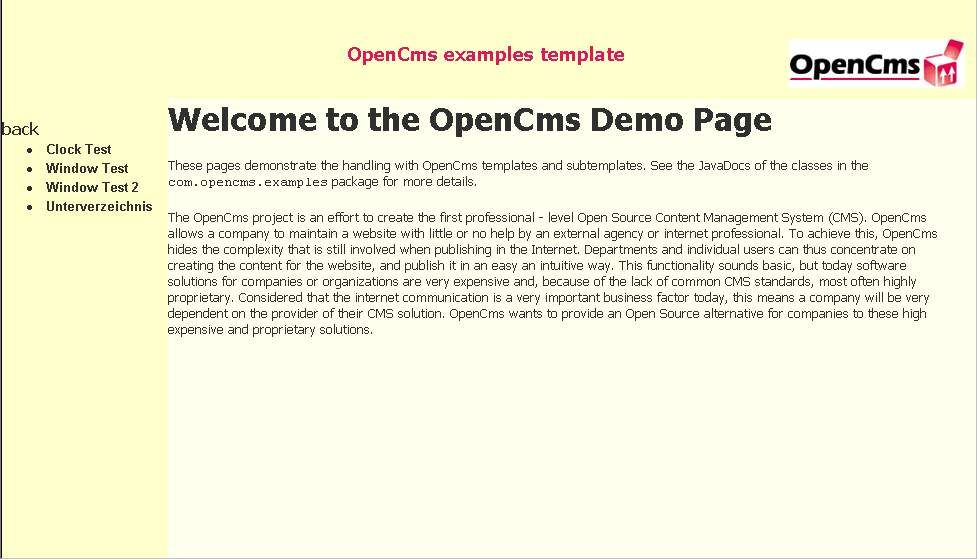
\includegraphics[width=\sgw]
                   {pics/usermanual/demoPage01}
\caption[Welcome page]
           {Welcome page}
\label{demopage01}
\end{center}
\end{figure}

\subsection{Editing a website}

Activate the "Workplace" to edit a page in OpenCms. The
"Workplace" is the OpenCms user interface that is used to change,
delete and create new pages. The "Workplace" is entirely based on
HTML, which is why you don't have to install additional software
to run it from your Internet browser.

Enter the following address in your browser to start the
"Workplace:"

{\tt http://localhost:8080/opencms/opencms/system/login/}

\subsubsection{Logging into the system}

In the login dialog box (Figure~\ref{loginbox}), enter "Admin" as
the user name and "admin" as the password.

\begin{figure}[!hbt]
\begin{minipage}[b]{0.35\linewidth}
   \begin{center}
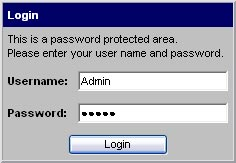
\includegraphics[width=\sgw]
                   {pics/usermanual/loginBox}
\caption["Login" dialog box]
           {"Login" dialog box}
\label{loginbox}
   \end{center}
\end{minipage}
\hfill
\end{figure}

Logging in automatically opens a new browser window and closes the
old one (you will be prompted to confirm this action). You are now
in the ``Workplace," in the so-called ``Explorer" view
(Figure~\ref{explorer}). This is where the actual editing starts.

\begin{figure}[!hbt]
\begin{center}

\includegraphics[width=\sgw]
                   {pics/usermanual/explorer}
\caption[Explorer view]
           {Explorer view}
\label{explorer}
\end{center}
\end{figure}

\textbf{NOTE:} OpenCms is a project based application, which means
that you cannot modify the pages online. You first have to create
an editing (offline) project. The default ``Offline" project can 
also be used for editing pages.

\subsubsection{Creating a new project}

Switch to the administration window by clicking on ``View" on the
menu bar and selecting ``Administration" from the drop-down menu
(Figure~\ref{view}).

\begin{figure}[!hbt]
\begin{center}
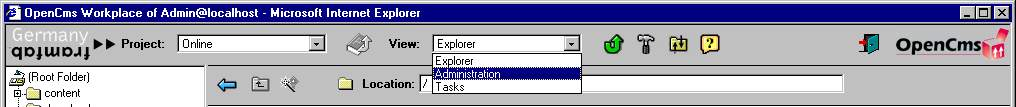
\includegraphics[width=\sgw]
                   {pics/usermanual/view}
\caption[Drop down menu ``View"]
           {Drop down menu ``View"}
\label{view}
\end{center}
\end{figure}

The Administration view is opened. The following buttons are
displayed: (Figure~\ref{adminview}):

\begin{figure}[!hbt]
\begin{center}
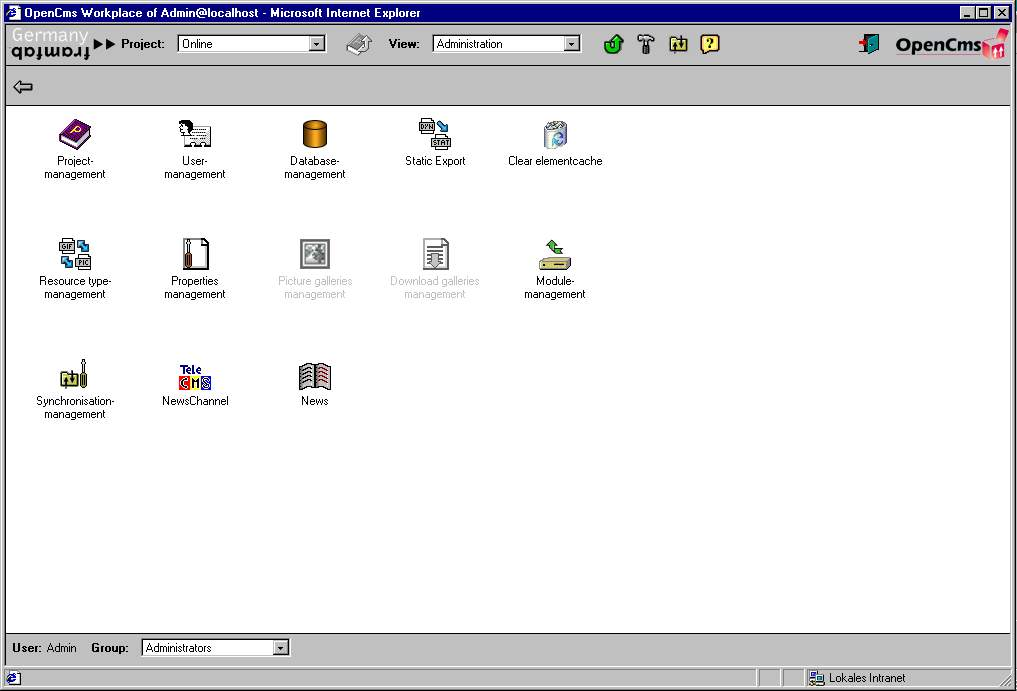
\includegraphics[width=\sgw]
                   {pics/usermanual/adminView}
\caption[``Administration" view]
           {``Administration" view}
\label{adminview}
\end{center}
\end{figure}

Click on ``Project Management." A new page is opened that contains
the following buttons (Figure~\ref{projectmanager}):

\begin{figure}[!hbt]
\begin{center}
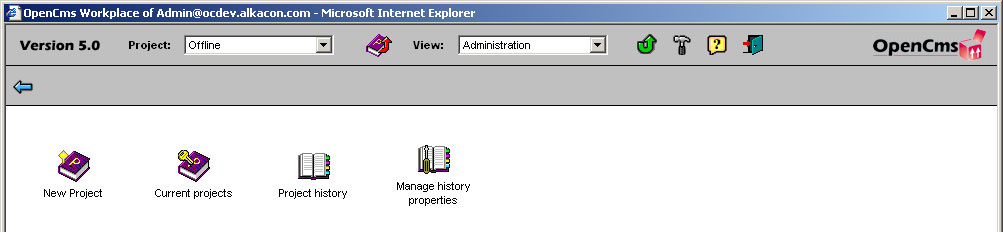
\includegraphics[width=\sgw]
                   {pics/usermanual/projectManager}
\caption[Project Management buttons]
           {Project Management buttons}
\label{projectmanager}
\end{center}
\end{figure}

Click on ``New Project" to create a new project.

The dialog window ``Create a new project" is opened
(Figure~\ref{createnewproject}). Enter the project data:

\begin{itemize}
\item Project name: Nice try
\item Description: Create test project
\item Folders: /release/
\item Channels: [leave empty]
\item User group: Users
\item Manager group: Project manager
\end{itemize}

Click on the "OK" button.

\textbf{NOTE:} Clicking on the folder icon next to the
``Directories" field opens a second window that contains a list of
the existing directories. Here you can select other directories for your
new project. The window closes automatically.

\begin{figure}[!hbt]
\begin{center}
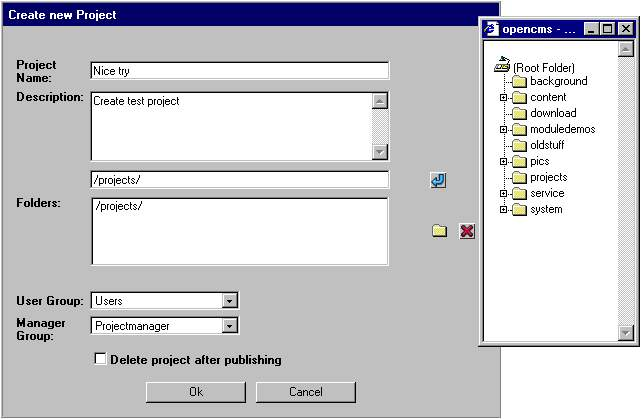
\includegraphics[width=\sgw]
                   {pics/usermanual/newProject}
\caption[Dialog window ``Create a new project"]
           {Dialog window ``Create a new project"}
\label{createnewproject}
\end{center}
\end{figure}

Switch back to the Explorer view by selecting it from the ``View"
drop-down menu. Select the ``/release/" directory (the same one you
selected when creating your project) from the drop-down menu. The
Explorer view is opened. Open your ``Nice try" project by selecting
it from the Project drop-down menu on the menu bar
(Figure~\ref{projectview}).

\begin{figure}[!hbt]
\begin{center}
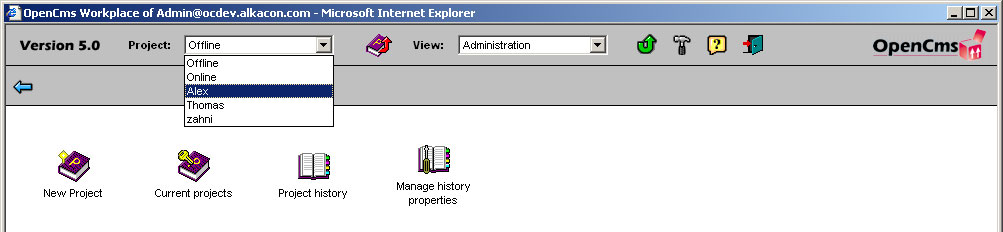
\includegraphics[width=\sgw]
                   {pics/usermanual/projectView}
\caption["Project" view]
           {"Project" view}
\label{projectview}
\end{center}
\end{figure}

The view for your project is open. You can now edit any one of its pages.

\textbf{NOTE:} You have surely noticed that all of the folders in
the folder tree are inactive except for ``/release/", ``/system/galleries/download/",
``/system/galleries/pics/", ``/system/galleries/externallinks/", 
``/system/galleries/htmlgalleries/" and ``/system/bodies/". 
Once the project is selected, OpenCms only allows you to modify files in your project directories.

\subsubsection{Editing pages}

A page must be locked for all other users before it can be opened.
Click on the icon next to the text "installation.html" with the left
mouse button to display the context-sensitive menu
(Figure~\ref{lockpage}). Click on the menu item "Lock."

\begin{figure}[!hbt]
\begin{center}
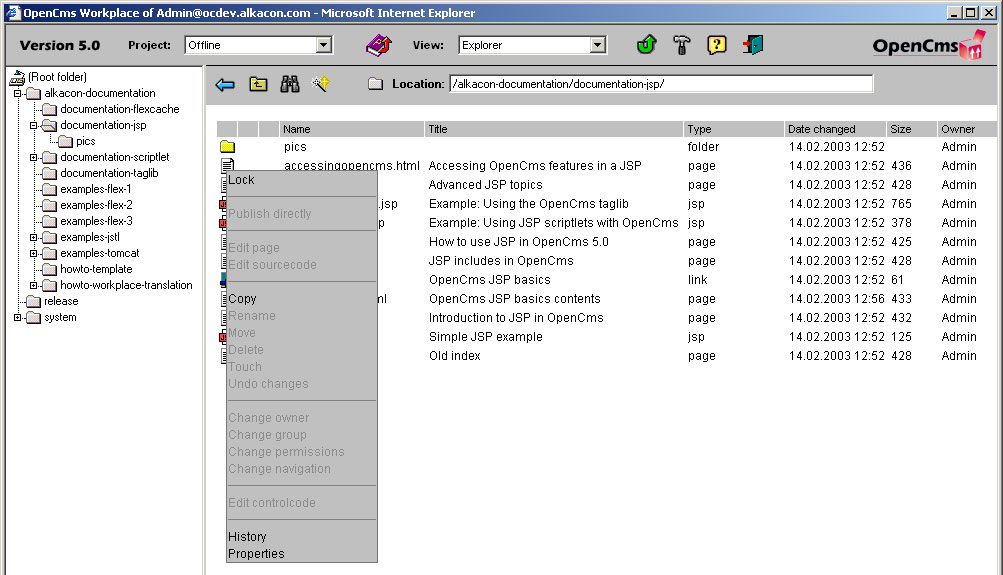
\includegraphics[width=\sgw]
                   {pics/usermanual/pageMenuUnlocked}
\caption[Context-sensitive menu]
           {Context-sensitive menu}
\label{lockpage}
\end{center}
\end{figure}

An open lock is displayed next to your locked file. Should the

\includegraphics{pics/usermanual/ic_locked}
icon not appear, check your browser settings (see above) or
refresh the view with the button

\includegraphics{pics/usermanual/ic_refresh}.

Click on the icon next to the text "installation.html" with the left
mouse button again to display the context-sensitive menu. Click on
"Edit page" to open the HTML editor.

\subsubsection{Working with the HTML editor}

You are now in the OpenCms HTML editor (Figure~\ref{htmleditor}).
Here you will find a number of editing icons that should be
familiar from other applications, such as Open Office or Word.

\begin{figure}[!hbt]
\begin{center}
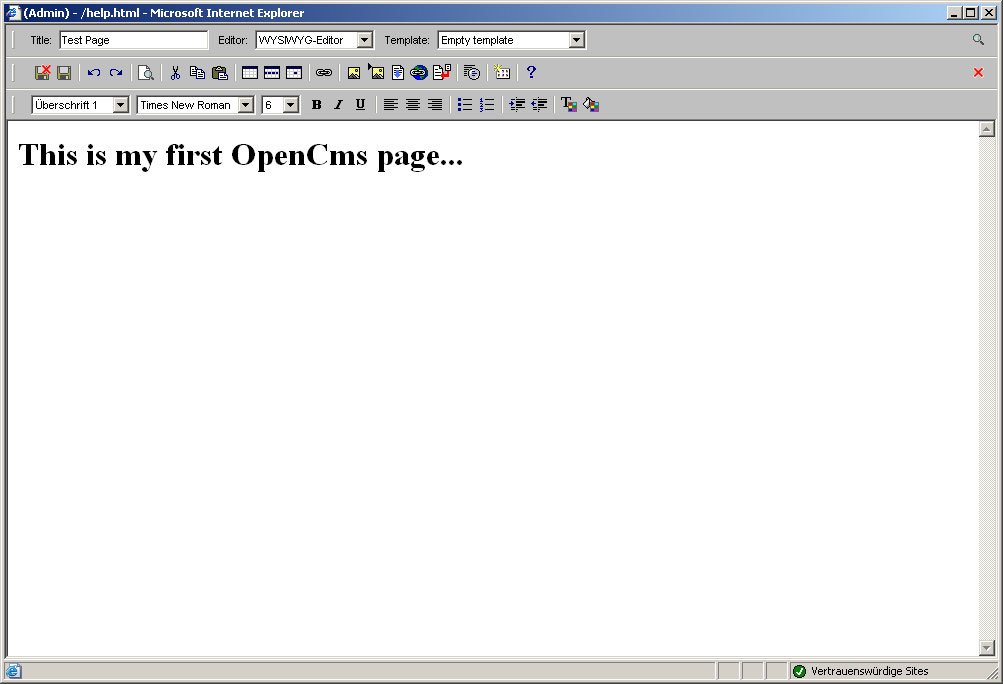
\includegraphics[width=\sgw]
                   {pics/usermanual/htmlEditor}
\caption[OpenCms HTML editor]
           {OpenCms HTML editor}
\label{htmleditor}
\end{center}
\end{figure}

In the text editor, which is just below the icons, the text that
you saw at the release notes page is
displayed. Make changes to the text and its format (e.g. bold, italics,
underline).

\textbf{By the way:} The HTML editor view you are currently in is
a WYSIWYG view (``\textbf{W}hat \textbf{y}ou \textbf{s}ee
\textbf{i}s \textbf{w}hat \textbf{y}ou \textbf{g}et"); this means
that pages are displayed here exactly as they will be seen later
on the Internet.

The "Template" drop-down menu is on the right part of the menu bar
(Figure~\ref{selecttemplate}). Select one of the pre-defined page
structures and layouts. You will see the changes by clicking on
the "preview" button in the upper right corner of the editor.

\begin{figure}[!hbt]
\begin{center}
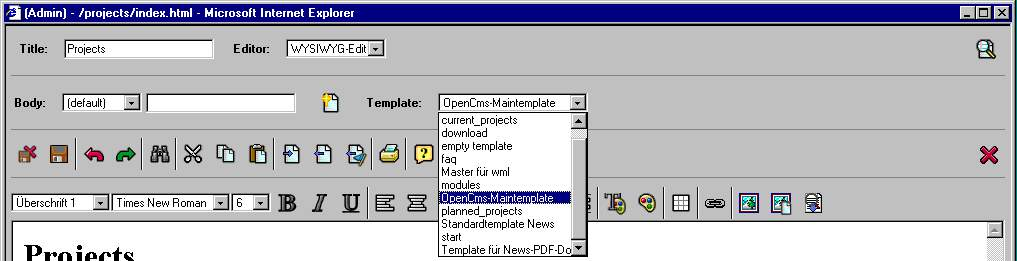
\includegraphics[width=\sgw]
                   {pics/usermanual/selectTemplate}
\caption[Drop-down menu "Template"]
           {Drop-down menu "Template"}
\label{selecttemplate}
\end{center}
\end{figure}

In the upper menu bar is the "Editor" drop-down menu, which
contains a selection of Editor views. You are currently in the
WYSIWYG view. Select the ``Sourcecode editor" view. The view is opened and
displays the same content as source code. Close the view by
clicking on the button ``Save \& Exit"

\includegraphics{pics/usermanual/ic_saveexit}, which is at the far
left of the menu bar.

The Explorer view is displayed.

\subsubsection{Completing the editing phase}

The page's details are currently displayed in red, which means
that the page has been edited. Additionally there is a little red
flag, which means that this page was locked and changed in the
current project. Click on the page icon of ``installation.html" with the left mouse to ``unlock" it. Click on
the menu item ``Unlock" in the context-sensitive menu to unlock the
page. The lock disappears (Figure~\ref{unlockpage}).

\begin{figure}[!hbt]
\begin{center}
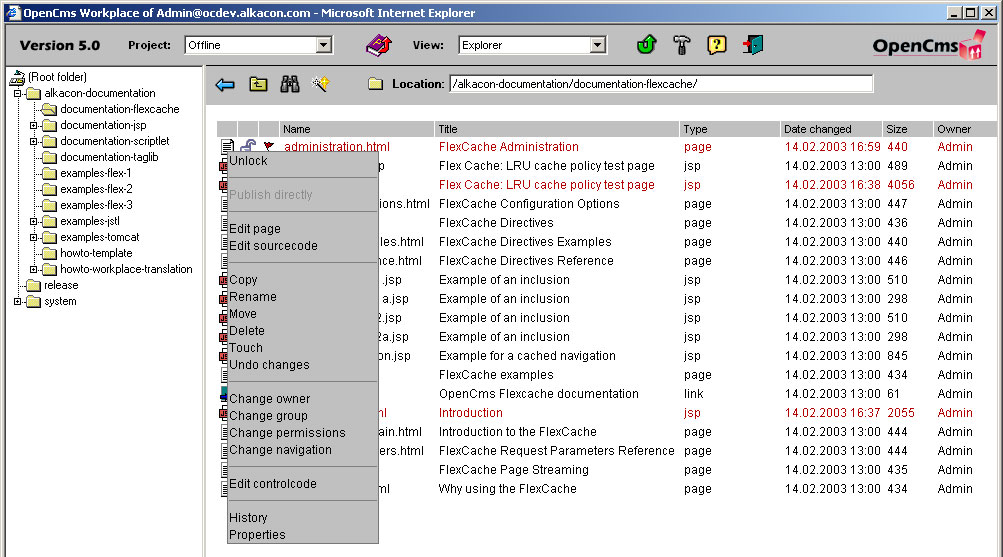
\includegraphics[width=\sgw]
                   {pics/usermanual/unlockPage}
\caption[Unlock an edited page]
           {Unlock an edited page}
\label{unlockpage}
\end{center}
\end{figure}

\subsubsection{Publishing a project}

Open the ``Administration" view. Click on the ``Project management"
button and after that on ``Current projects." The project you just edited
is displayed in the overview. Click on the project's icon to
access the context-sensitive menu. Select the menu item "Publish"
(Figure~\ref{publishproject}). Click on "OK."

\begin{figure}[!hbt]
\begin{center}
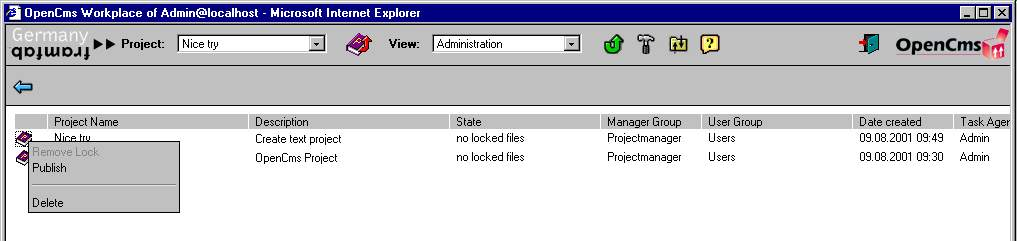
\includegraphics[width=\sgw]
                   {pics/usermanual/publishProject01}
\caption[Publishing a project]
           {Publishing a project}
\label{publishproject}
\end{center}
\end{figure}

\textbf{Note:} You can also publish the current project by clicking on the
icon between the project selector and the view selector on top of the OpenCms workplace.

Start the demo application again:\\
http://localhost:8080/opencms/opencms/release/installation.html.\\
The test page is displayed with your modifications (Figure~\ref{demopage02}).

\begin{figure}[!hbt]
\begin{center}
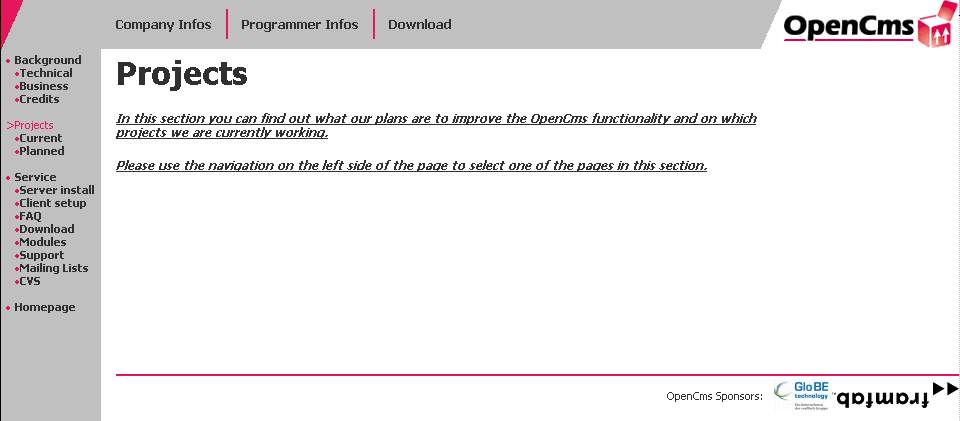
\includegraphics[width=\sgw]
                   {pics/usermanual/demoPage02}
\caption[Modified installation page]
           {Modified installation page}
\label{demopage02}
\end{center}
\end{figure}


\subsection{Creating a new page}

You can add new pages and folders for your web page from the
Explorer view. Create a new project or select the ``Nice try" project by following the steps
described above. Go to the ``/release/" directory by clicking on the
appropriate folder in the directory tree with the left mouse
button.

Click on the ``new" icon

\includegraphics{pics/usermanual/ic_newres}. The dialog window
``New" is opened (Figure~\ref{newpage01}).

Click on the radio button ``Page."

\begin{figure}[!hbt]
\begin{center}
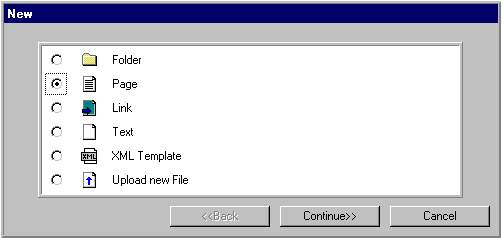
\includegraphics[width=\sgw]
                   {pics/usermanual/newPage01}
\caption[Dialog window ``New"]
           {Dialog window ``New"}
\label{newpage01}
\end{center}
\end{figure}

Click on the ``Continue" button. Enter the following data in the
dialog window ``Create a new page" (Figure~\ref{newpage02}):

\begin{itemize}
\item Name: help
\item Title: Test page
\item Template: Welcome / Release notes template
\item Keywords: Here you can enter some keywords
\item Description: Here you can enter a description
\item (Checkbox) add to navigation: check (default)
\item Text in Navigation: Help
\item Insert after: at the last position
\end{itemize}

\begin{figure}[!hbt]
\begin{center}
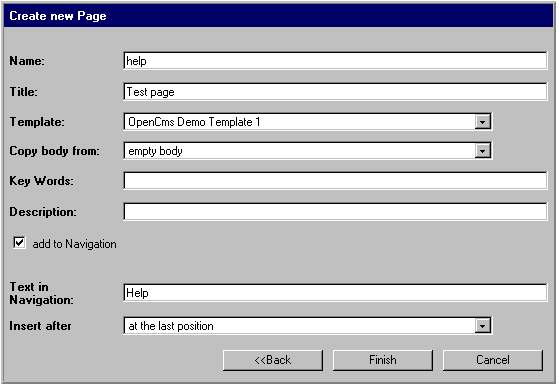
\includegraphics[width=\sgw]
                   {pics/usermanual/newPage02}
\caption[Dialog window ``Create a new page"]
           {Dialog window ``Create a new page"}
\label{newpage02}
\end{center}
\end{figure}

\textbf{NOTE:} The ``Text in navigation" is the name that will
later be displayed as the link in the online navigator.

Click on ``Finish". This takes you back to the Explorer view and
displays the details of your new page in blue with a lock
(Figure~\ref{explnewpage}). You can either continue editing the
page (see above) or use the context-sensitive menu to unlock it
for other users.

\begin{figure}[!hbt]
\begin{center}
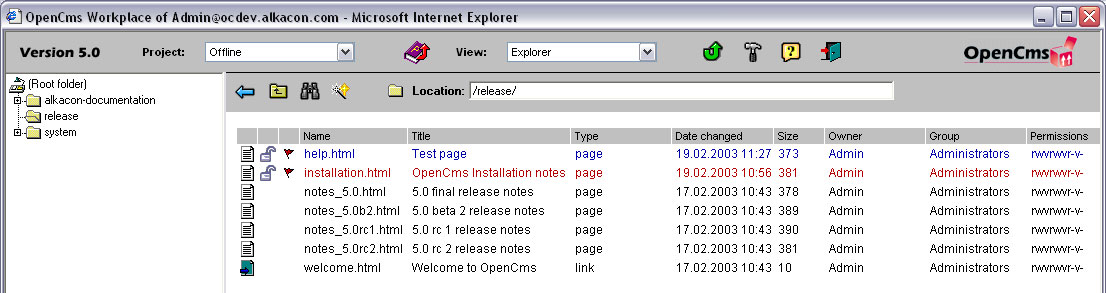
\includegraphics[width=\sgw]
                   {pics/usermanual/explNewPage}
\caption[Explorer view with new page]
           {Explorer view with new page}
\label{explnewpage}
\end{center}
\end{figure}

Publish the project as explained under ``Publishing a project" and
open the installation page:\\
http://localhost:8080/opencms/opencms/release/installation.html

The installation page is displayed with the new link to your page ``help.html" in the top navigation.
Click on the link to
view your new page (Figure~\ref{demopage03}). 

\begin{figure}[!hbt]
\begin{center}
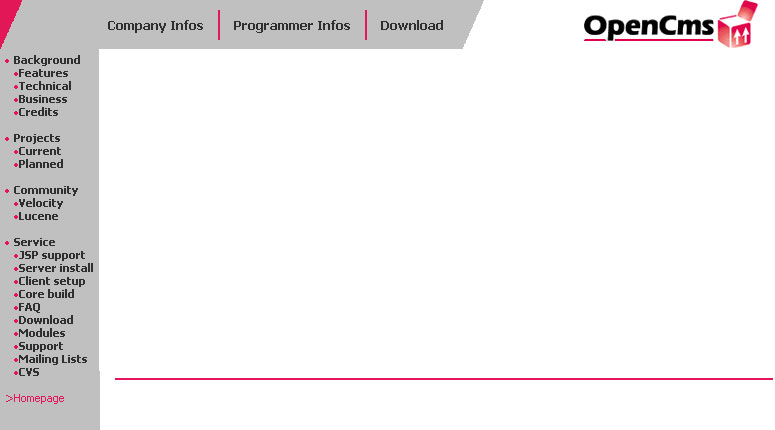
\includegraphics[width=\sgw]
                   {pics/usermanual/demoPage03}
\caption[New help page listed in navigation]
           {New help page listed in navigation}
\label{demopage03}
\end{center}
\end{figure}

This is the end of our short demo. Thank you for your attention. 
Additional and more detailed information about OpenCms is described in section 2 of the guide.

\newpage
\section{Section 2: OpenCms - The mechanics}

\subsection{The user interface}
The user interface is customized by clicking on the ``Settings" tab
(the ``hammer" button 
\includegraphics{pics/usermanual/ic_settings}
on the menu bar):

\begin{itemize}
\item The additional file information that is to be displayed in the Explorer view is defined on the ``Explorer" tab.
\item The Standard view and messaging options for task management are defined on the ``Tasks" tab.
\item The user's default startup settings and permissions for new files are defined on the ``Startup Options" tab.
\item A user's group and password are changed on the ``User Data" tab.
\end{itemize}

\subsection{View Modes}

The user screen contains all of the components, grouped in views,
that enable users to create, maintain and manage web pages. In the
``Explorer" view, users manage directories and files and edit HTML
pages. A project's workflow is managed in the ``Tasks" view. Users,
groups, projects, database connections, images, documents etc. are
managed in the ``Administration" view. The user screen (default
startup view) is started via a login dialog and is displayed as a
file explorer. The directory tree structure, the file view and the
menu bar make it easy for users to access files and functions
(Figure~\ref{workplace}) :

\begin{figure}[!hbt]
\begin{center}

\includegraphics[width=\sgw]
                   {pics/usermanual/workplace}
\caption[User screen]
           {User screen}
\label{workplace}
\end{center}
\end{figure}

Users can switch between the online version of the web page and
the individual offline projects by selecting one of the options in the
``Project" drop-down menu.

Users can switch between the ``Explorer", ``Tasks" and
``Administration" views by selecting one of the options in the
``View" drop-down menu.

The files and directories are managed via a context-sensitive menu
that is activated by clicking on the file or directory icon in the
file overview.

The content of the website as it will be seen online is displayed
in the browser screen (Figure~\ref{browserscreen}). The website's
files and directories cannot be modified in the online version.
The browser screen, which displays the page as it would be seen by
someone visiting the live site, is activated by clicking on the
file name in the ``Explorer" view:

\begin{itemize}
\item The Template of an OpenCms-generated browser page contains the
static and dynamic navigation components as well as other dynamic
components such as logos or text fields that can be freely
defined. The template determines the page's layout.
\item The content is displayed in the Body. Content is freely defined. Its
layout is based on previously defined format templates. The format
templates ensure that the content is uniformly displayed.
\end{itemize}

\begin{figure}[!hbt]
\begin{center}
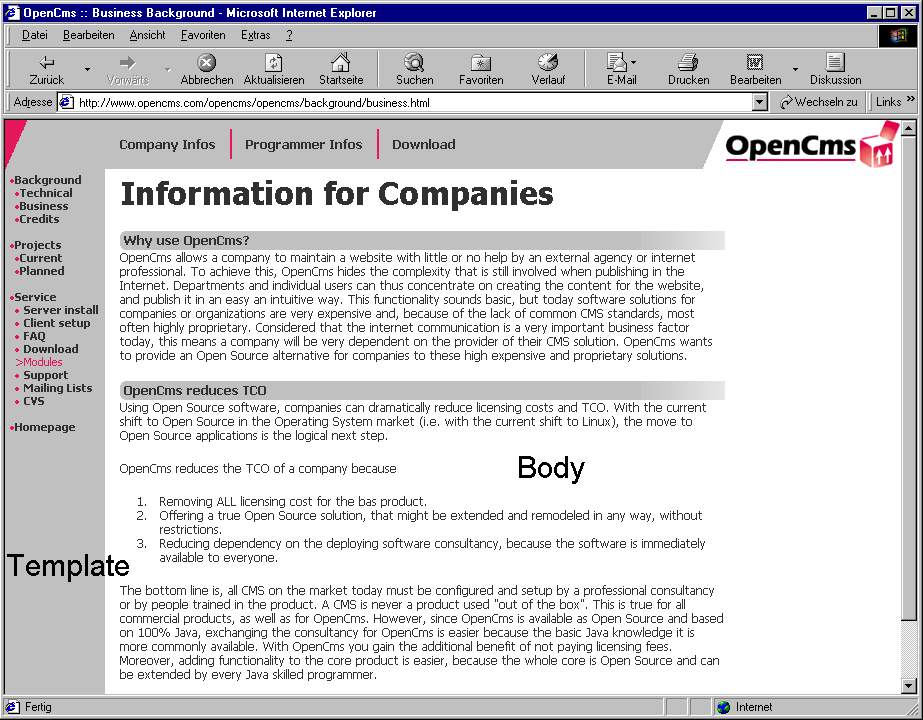
\includegraphics[width=\sgw]
                   {pics/usermanual/browserScreen}
\caption[Browser screen]
           {Browser screen}
\label{browserscreen}
\end{center}
\end{figure}

\subsection{Working on a project}

An offline project is created by a user that belongs to the
"Project manager" group. The project can be created for an
existing website that needs updating or a brand new website.

When you create an offline project for an existing website a view
on the offline resources for this website is created. When the
modified pages are published, the changes are copied to the online
project. Additionally the changed resources are stored in backup
tables for traceability purposes.

By default, an offline project's files and directories can only be
modified by the project members. Responsibilities are clearly
defined by assigning specific users and groups to specific files
and directories. It is also possible to process part of the web
site in different projects at the same time. Locking and unlocking
functions ensure that access security remains intact for larger
user groups.

The modifications that are made to the files are written to a
backup table after publishing. The information about all versions can
be accessed via the ``History" option in the context-sensitive menu
(Figure~\ref{history01}).

\begin{figure}[!hbt]
\begin{center}
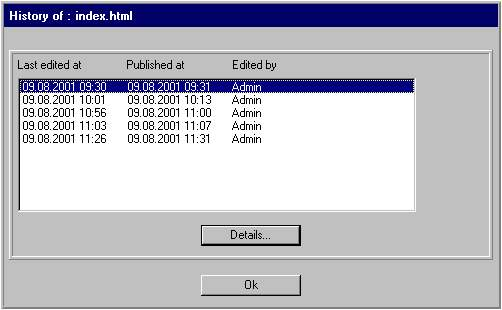
\includegraphics[width=\sgw]
                   {pics/usermanual/history01}
\caption[Project history]
           {Project history}
\label{history01}
\end{center}
\end{figure}

To create new content, the user creates a new file or directory by
clicking on the ``New" button on the menu bar. This opens a dialog
window in which the user selects the element to create: ``Folder,"
``Page," ``Link", ``Text", ``XMLTemplate", ``JSP" or ``Upload new file." The
name, title and navigation text as well as the position of the file
or directory in the navigation, are defined in separate dialog
boxes. Selecting the option ``Upload new file" enables users to load
files that are stored on their PC's local hard disks into an
OpenCms directory. Users access their assigned directories and
files via the file ``Explorer" view of OpenCms.

Clicking on the directory name (e.g. ``OpenCms") in the directory
tree structure or in the ``Explorer" view displays the directory's
contents. Clicking on an HTML file name (e.g. ``index.html") opens
a preview of the file in the Internet browser. Clicking on a directory or file
icon (text file, image etc.) in the file overview displays a
context-sensitive menu. The menu contains the following functions
that are accessible (active/inactive) based on the file's or
directory's status and the user's access permissions:

\begin{itemize}
\item \textbf{Lock or Unlock}: Directories or files can be locked throughout
the editing phase to prevent them from being accessed or modified
by several users at the same time. A file or directory is unlocked
when the user has finished modifying it.

\item \textbf{Publish directly}: A single resource can be published
directly. This item is enabled when a changed file is unlocked.

\item \textbf{Edit page}: Clicking opens a WYSIWYG editor in which the file can be modified.
At this stage, no HTML knowledge is required to modify a page.

\item \textbf{Edit sourcecode}: Clicking opens a text editor in which the file can be modified.
This requires at least basic HTML knowledge to modify a page.

\item \textbf{Edit control code}: Clicking opens a text editor in which
control codes can be edited.
\textbf{Warning:} Extensive knowledge of the OpenCms template mechanism is required
to make modifications of this type.

\item \textbf{History}: The history file displays all of the file's previous
versions. The history file enables users to see who made which
modifications when. When the file is locked a button for restoring
a version is shown in the ``Detail" of the version.

\item The respective access
attributes for the individual files and directories are set on the
system side by using the functions ``\textbf{Change owner}", ``\textbf{Change group}"
and ``\textbf{Change permissions}".

\item \textbf{Change navigation}: Here the navigation text and position of a resource can be changed.

\item \textbf{Properties}: To every resource properties can be attached as key / value pairs, 
e.g. the title or the description is stored as a resource property.
Properties can be added, modified or deleted.

\item Standard functions such as ``\textbf{Copy}",
``\textbf{Rename}", ``\textbf{Move}" and ``\textbf{Delete}" can be selected from the context
menus. ``\textbf{Touch}" changes the timestamp of a resource, which marks it as changed, 
and it will be published when the project is published.

\item \textbf{Undelete resources}: \index{undelete} When a resource
that already exists in the online project is deleted it is marked
by crossing out its entry in the file list. Now it is possible to
undelete these resources. When undeleting a folder all
subresources in this folder that were marked as deleted are
undeleted, too. You must have write access to undelete a resource.

\begin{figure}[!hbt]
\begin{center}
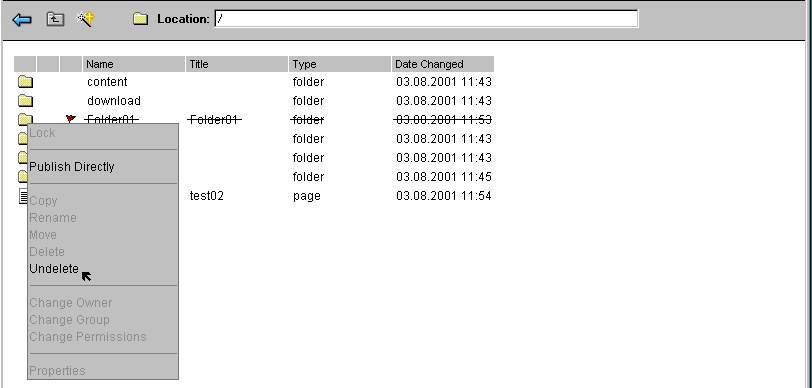
\includegraphics[width=\sgw]
                   {pics/newProject/undel03}
\caption[Undelete a resource]
           {Undelete a resource}
\label{undel}
\end{center}
\end{figure}

After the resource is undeleted its state is set to changed and
the resource is locked by the current user.


\item \textbf{Undo changes}  \index{undo}

Changes of a resource can be undone. The resource must be
marked as changed and it must be locked. You must have write
access to the resource. When the changes of a folder are undone
all changes of subresources are undone, too. This feature copies
the information from the online project, so all changes that were
not published yet are lost and new resources are deleted.

\begin{figure}[!hbt]
\begin{center}
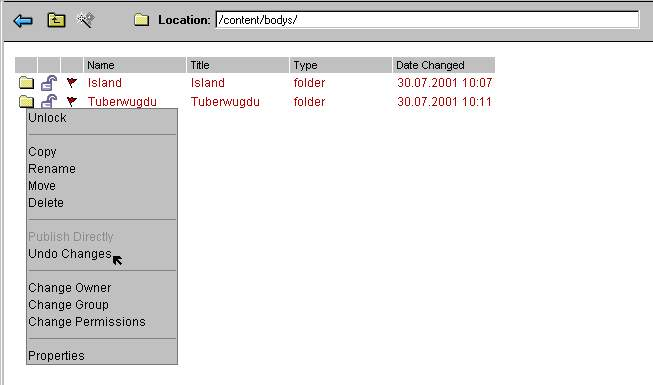
\includegraphics[width=\sgw]
                   {pics/newProject/undo01}
\caption[Undo changes of a resource]
           {Undo changes of a resource}
\label{undo}
\end{center}
\end{figure}


\item \textbf{Restore a version from history}  \index{history}

Older versions of a file can be restored from the history. The
file must be locked. This feature currently works only for files,
not for folders. The function is only enabled for locked files. It
is implemented in the detail view of the history.

You have to choose the version from the list of versions and click
on the detail button. To restore the version click on the ``Restore
version"-button. You must have write access to the file if you
want to restore a version.

\begin{figure}[!hbt]
\begin{minipage}[b]{0.49\linewidth}
\begin{center}
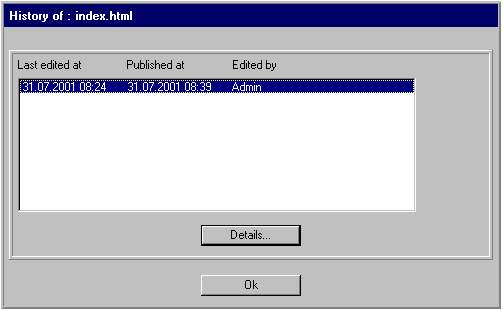
\includegraphics[width=\sgw]
                   {pics/newProject/restore01}
\end{center}
\end{minipage}
\begin{minipage}[b]{0.49\linewidth}
\begin{center}
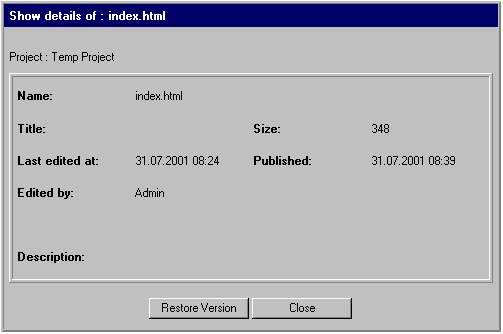
\includegraphics[width=\sgw]
                   {pics/newProject/restore02}
\end{center}
\end{minipage}
\caption[Restore a version]
           {Restore a version}
\label{restorever}
\end{figure}


\item \textbf{Publish a resource} \index{publish resource}

Resources can be published directly. They must be unlocked to
enable the function in the context menu. Only members of the projectmanager
and the administrator groups are allowed to publish resources of a project.

\begin{figure}[!hbt]
\begin{center}
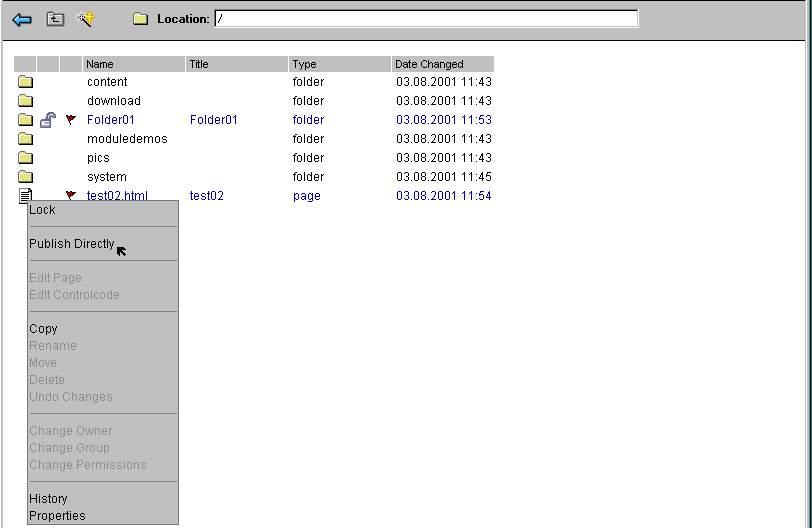
\includegraphics[width=\sgw]
                   {pics/newProject/publish03}
\caption[Publish a resource]
           {Publish a resource}
\label{publishres}
\end{center}
\end{figure}

When a resource is published directly

\begin{itemize}
\item a temporary project is created
\item the resource is copied to the new project
\item the projectid of the resource and all its subresources is set to the new project
\item the new project is published and deleted.
\end{itemize}


\item \textbf{Copy a resource to the project}

A resource that does not belong to the current offline project is
colored grey. You can copy this resource to the current offline
project with this new feature in the context menu. Only the
projectmanager and the administrator are allowed to copy resources
to the project.

\begin{figure}[!hbt]
\begin{center}
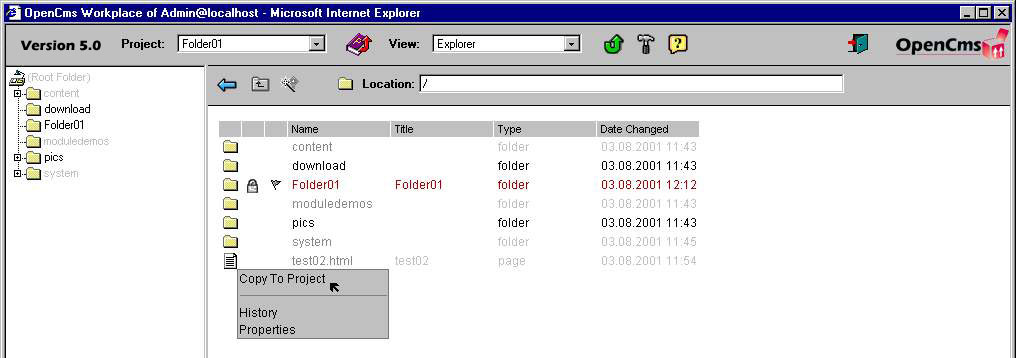
\includegraphics[width=\sgw]
                   {pics/newProject/copyPro02}
\caption[Copy a resource to project]
           {Copy a resource to project}
\label{copytoproject}
\end{center}
\end{figure}

You can also copy the parent resource of an already existing
resource to the project, but it is not possible to copy the root
folder to an existing project. For this you must create a new
project.

\end{itemize}

\subsection{Access permissions}

On the user side, different access permissions determine which
actions users can perform and which components they see, i.e.
users see only those files and directories that are relevant to
them. Doing this provides users with a well structured overview.
Each user belongs to at least one user group, but can belong to
several (Figure~\ref{newgroup}).

The following groups are pre-defined in OpenCms:

\begin{itemize}
\item \textbf{Administrators}: An administrator has full access permissions to
all of the files and directories. Administrators create and manage
users and user groups.
\item \textbf{Projectmanager}: A project manager creates new projects and coordinates their workflow. A project manager's access permissions are restricted to the projects he/she creates. A project manager can, however, access all of the files and directories within his/her projects. A project manager can also publish projects, i.e. put them online.
\item \textbf{Users}: A user can create new files and directories within the project he/she is assigned to. As the owner, the user has full access permissions to the files and directories he/she creates.
% \item \textbf{WebUsers}: Webusers cannot login in the OpenCms workplace, but can have access to restricted areas of a website which is forbidden for Guests.
\item \textbf{Guest}: This group consists of all other users, such as visitors.
\end{itemize}

Based on the requirements, additional groups such as editors,
designers, testers etc. can be created.

\begin{figure}[!hbt]
\begin{center}
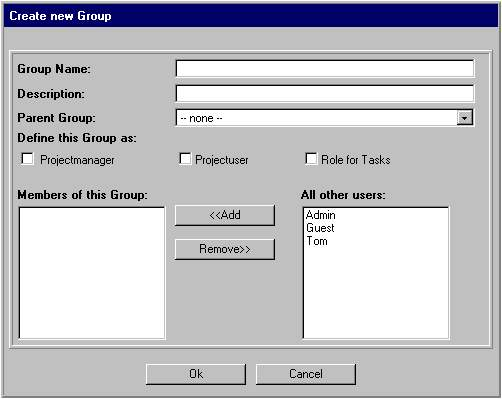
\includegraphics[width=\sgw]
                   {pics/usermanual/newGroup}
\caption[Create a new group]
           {Create a new group}
\label{newgroup}
\end{center}
\end{figure}

On the system side, each file and each directory is assigned to
one user, which by default, is the user that created the file or
directory, making him/her its owner. Each file and each directory
is also assigned to one user group that has specific access
permissions. This enables the users in this group to access the
files and directories that are relevant to them. File and/or
directory attributes, such as the owner of a file or directory, or
the group assigned to the files, can only be modified by the
administrator and/or the file and/or directory owner. All access
permissions are maintained via the ``Change owner", ``Change group"
and ``Change access permissions" options in the context
menu. File and directory access permissions are classified by
``Owner permissions", ``Group permissions" and ``Other permissions." A
user's access permission can be restricted to the files and
directories that he/she owns. The following abbreviations are used
to set a user's permissions: r = read, w = write, v = visible, i =
internal.

\subsection{The editor}

The editor is used to create content in the body, which is
structured by a template that ensures that the layout for the
navigator, the content and the individual pages - basically the
layout for the whole site - is uniform
(Figure~\ref{thehtmleditor}):

\begin{figure}[!hbt]
\begin{center}
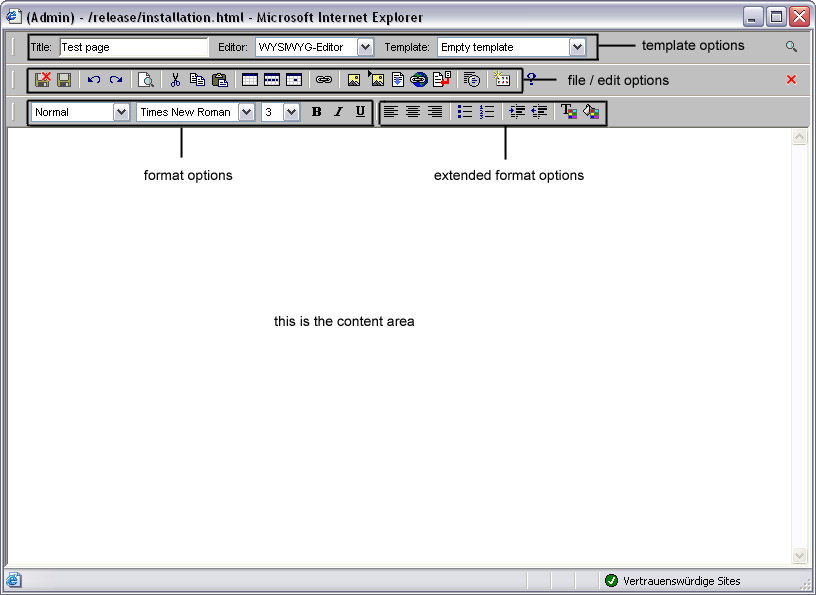
\includegraphics[width=\sgw]
                   {pics/usermanual/theHtmlEditor}
\caption[The HTML editor]
           {The HTML editor}
\label{thehtmleditor}
\end{center}
\end{figure}

The functionality of the OpenCms editor is very similar to that of
a standard WYSIWYG HTML editor with templates, tables and preview
functions, such as Netscape Composer. It is also possible to
switch between sourcecode and WYSIWYG mode. A page's layout is
determined by a template. Complex layouts are created by cascading
several templates. The editor in OpenCms is only used to edit the body of an HTML page.

\subsection{Workflow}

The project manager creates a new task and defines its role by
clicking on the ``New" button in the ``Tasks" view. A role consists
of several users that have the skills to perform a specific task
such as editing, designing graphics, writing HTML code, etc. A
preferred user is selected for each task. The name, the
definition, the due date and the priority of the task as well as
various messaging options are also defined. Depending on the
selected messaging options, an e-mail is automatically sent to
either the preferred user or all users that are assigned to a role
as soon as a new task has been added to the project. The task is
active once the appropriate user has accepted it. Optionally, the
project manager receives an e-mail when the task has been
accepted, rejected, forwarded or completed. Users can view the
tasks that have been assigned to them as well as those they have
forwarded to others by filtering on specific criteria in the
drop-down menu ``Filter" (Figure~\ref{taskview}). Different icons
and colors are also used to define a project's status. A task that
is still within the due date is shown in black. If the due date is
exceeded, the task is shown in red. A completed task is shown in
gray. A task's priority is defined by icons (low, normal and
high). The task descriptions provide a clear overview of a user's
task account.

\begin{figure}[!hbt]
\begin{center}
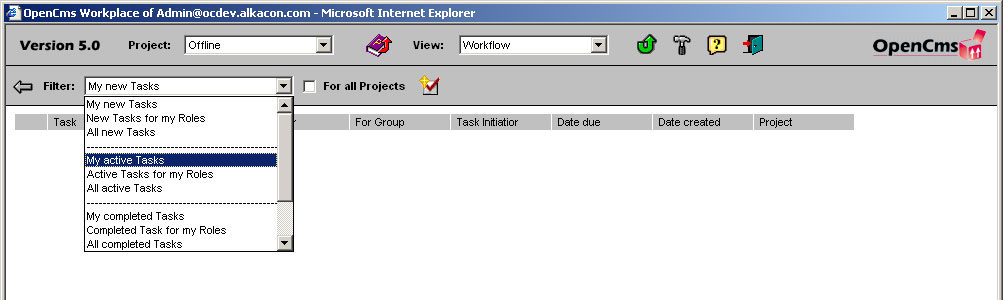
\includegraphics[width=\sgw]
                   {pics/usermanual/taskView}
\caption["tasks" view]
           {"tasks" view}
\label{taskview}
\end{center}
\end{figure}

Clicking on the name of a new task displays its details and
history. Each stage of the project is tracked and ensures that the
workflow remains transparent.
